% ====================================================================
%  KANDA — IEEE Conference Paper
%  "KANDA: Hardware-Aware LLM-Driven Navigation on Commodity IoT Hardware"
%  IEEE two-column conference format
%  Compile with: pdflatex → bibtex → pdflatex × 2
% ====================================================================
\documentclass[conference]{IEEEtran}
\IEEEoverridecommandlockouts

% ---------- PACKAGES ----------
\usepackage{cite}
\usepackage{amsmath,amssymb,amsfonts}
\usepackage{algorithm}
\usepackage{algorithmic}
\usepackage{graphicx}
\usepackage{textcomp}
\usepackage{xcolor}
\usepackage{booktabs}
\usepackage{array}
\usepackage{tabularx}
\usepackage{multirow}
\usepackage{enumitem}
\usepackage{listings}
\usepackage{float}
\usepackage{tikz}
\usepackage[hidelinks]{hyperref}
\usetikzlibrary{shapes.geometric,arrows.meta,positioning,calc,backgrounds,fit}

\lstset{
  basicstyle=\ttfamily\scriptsize,
  breaklines=true,
  breakatwhitespace=false,
  frame=single,
  numbers=none,
  captionpos=b,
  aboveskip=6pt,
  belowskip=2pt,
  belowcaptionskip=2pt,
  keepspaces=true,
  columns=flexible,
  keywordstyle=\color{blue!70!black},
  commentstyle=\color{green!50!black},
  stringstyle=\color{red!60!black},
}

\def\BibTeX{{\rm B\kern-.05em{\sc i\kern-.025em b}\kern-.08em
    T\kern-.1667em\lower.7ex\hbox{E}\kern-.125emX}}

% ====================================================================
\begin{document}

\title{KANDA: Hardware-Aware LLM-Driven Autonomous Navigation\\
on Commodity IoT Hardware with Runtime Safety Enforcement}

\author{%
\IEEEauthorblockN{Sudarshan T S}
\IEEEauthorblockA{%
\textit{Dept.\ of Information Science and Engineering}\\
\textit{RV College of Engineering (Autonomous)}\\
Bengaluru 560059, India\\
\texttt{1RV24SIT14@rvce.edu.in}}
\and
\IEEEauthorblockN{Sushmitha N}
\IEEEauthorblockA{%
\textit{Dept.\ of Information Science and Engineering}\\
\textit{RV College of Engineering (Autonomous)}\\
Bengaluru 560059, India\\
\texttt{sushmitha@rvce.edu.in}}
}

\maketitle

% ====================================================================
\begin{abstract}
We designed, built, and validated \textbf{KANDA} (Knowledge-driven Autonomous
Navigation and Decision-making Agent), a differential-drive mobile robot that
integrates a cloud large language model into a hard real-time embedded control
loop on commodity IoT hardware under \$60.
Coupling an LLM to a physical motor controller exposes three concrete
engineering problems absent from purely software deployments: the model has no
inherent knowledge of the robot's actuator vocabulary, speed limits, or sensor
geometry (\emph{semantic grounding}); raw model output may be structurally
invalid for MCU firmware to parse (\emph{output reliability}); and cloud
inference round-trips of 1.5--4.2\,s are incompatible with the sub-100\,ms
obstacle-response window required for safe navigation
(\emph{timing decoupling}).

We address all three through a co-designed three-layer stack.
A \emph{hardware-aware prompt} encodes the robot's complete action vocabulary,
speed bounds, sensor axes, and numeric proximity safety thresholds into every
inference request, anchoring model outputs within physical actuator affordances
before any decoding occurs.
A \emph{structured JSON command contract} restricts model output to a
seven-element motion vocabulary with a single integer speed field, making every
response directly dispatchable by the ESP32 firmware without further parsing
beyond \texttt{strcmp}.
A \emph{deterministic safety validator} on the Raspberry Pi edge node enforces
an action whitelist, coerces and clamps speed to $[0,255]$, and substitutes a
hard stop on any violation, ensuring no unvalidated model output reaches the
motor driver regardless of cloud or network state.

The system implements a three-tier IoT device--edge--cloud
pipeline~\cite{bonomi2012fog,shi2016edge}: an ESP32 DevKit (dual-core Xtensa,
240\,MHz) handles real-time HC-SR04 ranging and TB6612FNG H-bridge actuation;
a Raspberry Pi 3B+ runs the Python intelligence stack and safety validator
locally; Google Gemini~2.5 Flash~\cite{gemini2023report} provides language
reasoning via HTTPS.
Dual-mode firmware on the ESP32 realises Brooks's subsumption
principle~\cite{brooks1986robust} on a \$4 microcontroller: AI\_MODE when
the edge node supplies validated commands; autonomous rule-based AUTO\_MODE
via a 5\,s watchdog when it does not.
The two processors communicate exclusively over a UART link at
115,200\,baud using newline-framed ASCII messages.
Dual-mode firmware on the ESP32 provides continuous autonomous collision
avoidance when the edge node is silent, reverting via a 5\,s watchdog
to rule-based AUTO\_MODE—implementing Brooks's subsumption principle on a
\$4 microcontroller.

The complete hardware bill of materials totals under \$60.
Bench demonstrations across three scenario classes and four fault
conditions confirm that hardware-aware prompting produces contextually
appropriate commands while the validation layer prevents unsafe actuation
in every tested failure mode.
A controlled prompt ablation study quantifies a 30\% increase in
invalid-command rate when the action vocabulary is removed, and a 20\% increase
in unsafe forward commands when proximity safety rules are removed,
confirming that specification-level and runtime alignment layers address
orthogonal failure modes and are jointly necessary.
\end{abstract}

\begin{IEEEkeywords}
embodied AI, hardware-aware prompting, LLM robot control, safety validation,
ESP32, Raspberry Pi, Gemini~2.5, IoT edge-cloud, dual-mode firmware,
sense--reason--act, autonomous obstacle avoidance
\end{IEEEkeywords}

% ====================================================================
\section{Introduction}
\label{sec:intro}
% ====================================================================

Low-cost differential-drive platforms built around ESP32- or Arduino-class
microcontrollers have become the workhorse of indoor navigation and logistics
automation~\cite{ifr2024report,atzori2010iot}.
Their embedded firmware typically implements a finite-state machine keyed on
fixed distance thresholds: if the front sensor reads below $d_{f}$, pivot;
if a side sensor reads below $d_{s}$, arc away.
This architecture is deterministic and computationally inexpensive, yet it
is brittle: it cannot reason about novel obstacle configurations, cannot
interpret ambiguous spatial cues, and requires manual firmware extension for
every new scenario.
A robot navigating a corridor with asymmetrically placed obstacles---a
configuration its programmer never anticipated---has no mechanism to
\emph{reason} about the situation; it oscillates between conflicting rules
or stalls.

Recent advances in Large Language Models (LLMs)~\cite{brown2020gpt3,
openai2023gpt4, gemini2023report} suggest an alternative: describe the robot's
sensor state in natural language and ask the model for a contextually
appropriate action.
Foundational research in embodied AI---PaLM-E~\cite{driess2023palme},
SayCan~\cite{ahn2022saycan}, RT-2~\cite{brohan2023rt2}, and
RT-1~\cite{brohan2022rt1}---demonstrates that LLMs and vision-language models
can ground language understanding in physical affordances, enabling task
planning and even direct action generation for robotic manipulation.
Inner Monologue~\cite{huang2022innermonologue} and
ReAct~\cite{yao2023react} further showed that closed-loop reasoning---where
environment feedback updates the model's context at each step---enables dynamic
replanning, directly motivating KANDA's sense--reason--act pipeline.

However, all of these systems operate on research-grade hardware costing
thousands to millions of dollars, or require cloud-scale training pipelines.
Three engineering problems separate raw LLM capability from deployable robot
intelligence on commodity IoT hardware:

\textbf{P1 --- Semantic grounding.}
A general-purpose language model has no inherent knowledge of a specific
robot's actuator vocabulary, speed range, or sensor axes.
Without an explicit hardware description, the model generates
physically impossible commands or prose instructions that firmware cannot
parse~\cite{ahn2022saycan, vemprala2024chatgpt}.

\textbf{P2 --- Output structure.}
Even a well-prompted model occasionally wraps its response in markdown fencing,
expresses a numeric speed as a float string, or introduces a typo in an action
name.
Feeding raw model output directly to a microcontroller motor driver is unsafe.

\textbf{P3 --- Timing decoupling.}
Ultrasonic collision detection requires sub-100\,ms reaction times.
Cloud LLM round-trips average 1.5--4\,s.
A control architecture that stalls waiting for an LLM reply during an
obstacle approach will collide~\cite{brooks1986robust}.

The broader IoT and edge-computing literature frames this as the
\emph{device--edge--cloud} continuum~\cite{bonomi2012fog, shi2016edge}:
latency- and safety-critical computation belongs on the device or edge node;
flexible reasoning that tolerates latency belongs in the cloud.
TinyML research~\cite{warden2020tinyml, david2021tflitemicro, lin2020mcunet}
demonstrates that microcontrollers can execute quantised ML models, but
current LLM sizes far exceed embedded flash constraints, reinforcing the
edge-offload pattern for language reasoning.

\textbf{KANDA} (Knowledge-driven Autonomous Navigation and Decision-making
Agent) addresses all three problems through a layered design on commodity IoT
components totalling under \$60.

\subsection*{Contributions}
\begin{enumerate}[leftmargin=*, nosep]
  \item A complete dual-processor IoT architecture for LLM-driven mobile
        robots, reproducible from commodity components at under \$60.
  \item A \emph{hardware-aware prompt design methodology} that aligns LLM
        outputs with physical actuator affordances via specification-level,
        decoding-level, and runtime alignment---without fine-tuning.
  \item A \emph{layered safety framework} (prompt contract + JSON schema +
        deterministic validator) that guarantees a finite, bounded, whitelisted
        command always reaches the motor driver regardless of model behaviour.
  \item \emph{Dual-mode firmware} implementing Brooks's subsumption
        principle~\cite{brooks1986robust} on a \$4 microcontroller:
        LLM-driven in AI\_MODE when the edge node is healthy;
        autonomous rule-based avoidance in AUTO\_MODE when it is not.
  \item Empirical evaluation across three navigation scenarios and four
        injected fault conditions, with a prompt ablation study that
        quantifies the contribution of each alignment layer.
\end{enumerate}

The rest of the paper: Section~\ref{sec:related} surveys related work;
Section~\ref{sec:arch} describes the architecture;
Section~\ref{sec:methodology} presents the full methodology;
Section~\ref{sec:results} reports results;
Section~\ref{sec:discussion} discusses limitations and future work;
Section~\ref{sec:conclusion} concludes.

% ====================================================================
\section{Related Work}
\label{sec:related}
% ====================================================================

\subsection{LLMs for Robot Planning and Control}

SayCan~\cite{ahn2022saycan} established the key principle that language
plausibility alone is insufficient for robot control: affordance grounding
is required to select actions that are both useful and physically feasible.
KANDA realises this through explicit prompt specification rather than learned
value functions, eliminating the need for a demonstration dataset.

RT-1~\cite{brohan2022rt1} trains a dedicated robotics transformer on 130,000
demonstrations; RT-2~\cite{brohan2023rt2} fine-tunes a vision-language model
on robot trajectories to generate action tokens.
PaLM-E~\cite{driess2023palme} embeds continuous sensor observations into a
562B-parameter multimodal model.
All require research-scale hardware and datasets; KANDA achieves LLM-driven
control via API inference alone, following the prompt-engineering discipline
established by Vemprala et al.~\cite{vemprala2024chatgpt}.

Huang et al.~\cite{huang2022zeroshot} showed that LLMs can produce
physically grounded action sequences without robot-specific fine-tuning,
validating KANDA's inference-only deployment.
Inner Monologue~\cite{huang2022innermonologue} closes the sense--reason--act
loop with environment feedback; ReAct~\cite{yao2023react} interleaves
reasoning traces and actions.
KANDA is a constrained instantiation where the action space is finite and
execution is physical.
Wei et al.'s chain-of-thought work~\cite{wei2022cot} motivates KANDA's
structured hardware preamble as an analogue of providing the model with
explicit reasoning context.

Liang et al.~\cite{liang2023code} generate robot control code;
Singh et al.~\cite{singh2023progprompt} generate situated task programs.
KANDA targets single-step JSON commands---simpler but more tractable for
MCU firmware parsing.
Huang et al.~\cite{huang2023grounded} modify per-token probabilities at
decode time; KANDA applies the complementary post-generation approach via a
deterministic validator.
Shah et al.~\cite{shah2022lmnav} combine CLIP, GPT-3, and a navigation model
for topological outdoor navigation---the closest published system to KANDA's
Phase~3 goals.

\subsection{Safety in AI-Driven Systems}

Amodei et al.~\cite{amodei2016safety} catalogue concrete AI safety problems
including specification gaming and safe exploration.
KANDA's whitelist-plus-clamp validator is a runtime instance of their
specification-gaming countermeasure: the system cannot learn to exploit an
action that does not exist in the whitelist.

\subsection{Layered Robot Control}

Brooks~\cite{brooks1986robust} organises robot behaviours in layers, with
reactive behaviours subsuming deliberative ones.
KANDA is a direct implementation: the ESP32 reactive layer runs at
$\sim$10\,Hz; the Raspberry Pi deliberative layer at 0.5\,Hz;
the 5\,s watchdog implements subsumption by reverting to the reactive
layer when the deliberative layer is silent.
The Dynamic Window Approach~\cite{fox1997dwa} provides the classical
background for the AUTO\_MODE obstacle-avoidance logic KANDA's firmware
implements.

\subsection{IoT Edge-Cloud and TinyML}

The fog-computing model~\cite{bonomi2012fog} and the edge vision of Shi et
al.~\cite{shi2016edge} establish that safety-critical computation should
reside at the edge rather than in the cloud.
KANDA's Pi edge node executes the safety validator locally, ensuring a
cloud failure never results in unsafe actuation.
The foundational IoT survey of Atzori et al.~\cite{atzori2010iot} provides
the architectural vocabulary for KANDA's three-tier device--edge--cloud model.
Wireless sensor network theory~\cite{akyildiz2002wsn} underpins the
HC-SR04 echo-timing model.
Murshed et al.~\cite{murshed2022edge} survey ML at the network edge;
Warden and Situnayake~\cite{warden2020tinyml}, David et al.~\cite{david2021tflitemicro},
and Lin et al.~\cite{lin2020mcunet} provide the technical foundations for
on-device ML on ESP32-class hardware that motivates KANDA's Phase~4 roadmap.

% ====================================================================
\section{System Architecture}
\label{sec:arch}
% ====================================================================

\subsection{Three-Tier IoT Architecture}

KANDA follows the device--edge--cloud model~\cite{bonomi2012fog, shi2016edge},
as illustrated in Fig.~\ref{fig:arch}.

\begin{figure}[t]
\centering
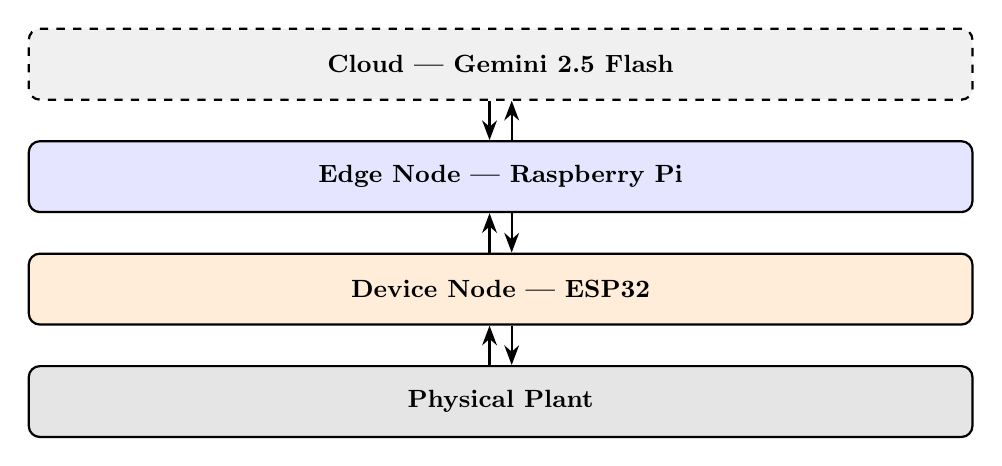
\begin{tikzpicture}[
  box/.style={draw, thick, rounded corners=4pt,
              minimum width=\columnwidth-4pt, minimum height=0.9cm,
              align=center, font=\small\bfseries},
  arr/.style={-{Stealth[length=2.5mm]}, thick},
  node distance=0.5cm
]
\node[box, fill=gray!12, dashed] (cloud) {Cloud --- Gemini 2.5 Flash};
\node[box, fill=blue!10,  below=of cloud] (pi)   {Edge Node --- Raspberry Pi};
\node[box, fill=orange!15, below=of pi]   (esp)  {Device Node --- ESP32};
\node[box, fill=gray!20,  below=of esp]   (phys) {Physical Plant};
\draw[arr, transform canvas={xshift= 4pt}]
  (pi.north)  -- (cloud.south);
\draw[arr, transform canvas={xshift=-4pt}]
  (cloud.south) -- (pi.north);
\draw[arr, transform canvas={xshift= 4pt}]
  (pi.south)  -- (esp.north);
\draw[arr, transform canvas={xshift=-4pt}]
  (esp.north) -- (pi.south);
\draw[arr, transform canvas={xshift= 4pt}]
  (esp.south)  -- (phys.north);
\draw[arr, transform canvas={xshift=-4pt}]
  (phys.north) -- (esp.south);
\end{tikzpicture}
\caption{Three-tier IoT architecture of KANDA.}
\label{fig:arch}
\end{figure}

\textbf{Cloud tier.}
Gemini~2.5 Flash handles language-conditioned decision-making via HTTPS.
Its outputs are bounded to 64 tokens at temperature~0.2.

\textbf{Edge tier (Raspberry Pi).}
Hosts all Python intelligence modules.
The safety validator executes \emph{locally} before any command is sent,
ensuring cloud failure causes a locally-generated stop rather than silence.

\textbf{Device tier (ESP32).}
Runs a tight real-time loop: sample sensors, transmit telemetry, receive and
parse JSON, drive motors, update OLED.
Reverts to rule-based AUTO\_MODE after 5\,s of UART silence.

\subsection{Hardware Specification}

\begin{table}[t]
\caption{Hardware components and key parameters}
\label{tab:hw}
\centering
\renewcommand{\arraystretch}{1.05}
\begin{tabular}{@{}p{2.0cm}p{2.8cm}p{2.4cm}@{}}
\toprule
\textbf{Component} & \textbf{Role} & \textbf{Key pins / notes} \\
\midrule
ESP32 DevKit    & MCU at 240\,MHz & 38-pin dual-core \\
Raspberry Pi 3B+& Edge intelligence & \texttt{/dev/ttyS0} \\
TB6612FNG       & Dual H-bridge, 1\,kHz PWM & AIN1/2: 18/19; PWMA: 23 \\
HC-SR04$\times$3& Front/left/right ranging & TRIG: 5/13/4; ECHO: 34/35/32 \\
SSD1306 OLED    & 128$\times$64 I$^2$C display & SDA: 21, SCL: 22 \\
Voltage dividers& 5\,V ECHO $\to$ 2.5\,V & 1k+1k$\Omega$ \\
LiPo 7.4\,V+BMS & Primary battery & $\to$ buck $\to$ 5\,V rail \\
\bottomrule
\end{tabular}
\end{table}

ECHO pins GPIO~34 and~35 are input-only with no boot-strapping role,
preventing unintended boot-mode changes.
Resistor dividers reduce 5\,V HC-SR04 ECHO signals to $\approx$2.5\,V,
within the ESP32's 3.3\,V GPIO absolute-maximum
tolerance~\cite{espressif2023esp32}.

\begin{figure}[t]
\centering

\includegraphics[width=\columnwidth]{kanda_robot.png}
\caption{KANDA prototype: ESP32 (left), Raspberry Pi (centre),
HC-SR04 sensors (front/sides), and TB6612FNG motor driver (rear).}
\label{fig:proto}
\end{figure}

\subsection{UART Serial Protocol and Control Cycle}

Two message types traverse the UART link:

\textbf{Telemetry (ESP32 $\to$ Pi):}
\texttt{F:\textit{ff.f} L:\textit{ll.l} R:\textit{rr.r} -> \textit{LABEL}}

\textbf{Command (Pi $\to$ ESP32):}
\texttt{\{"action":"slight\_left","speed":110\}}

One complete control cycle executes in seven steps:
\emph{(1)}~three ultrasonic pings ($<$100\,ms total);
\emph{(2)}~telemetry line transmitted ($<$5\,ms);
\emph{(3)}~Pi parses, builds prompt, queries Gemini (1.5--4.2\,s);
\emph{(4)}~safety validator inspects response ($<$1\,ms);
\emph{(5)}~Pi transmits one JSON command line ($<$5\,ms);
\emph{(6)}~ESP32 parses JSON, drives TB6612FNG, updates OLED;
\emph{(7)}~Pi sleeps 2\,s; ESP32 continues sensing and may revert to
AUTO\_MODE if no JSON arrives within 5\,s.
The firmware inner loop ($\sim$10\,Hz) is two orders of magnitude faster than
the intelligence outer loop (0.5\,Hz), satisfying the timing-decoupling
requirement (P3) by construction.

% ====================================================================
\section{Methodology}
\label{sec:methodology}
% ====================================================================

KANDA's methodology realises the three-layer alignment
strategy~\cite{huang2023grounded}: \emph{specification-level} (hardware-aware
prompt), \emph{decoding-level} (temperature and token budget), and
\emph{runtime} (safety validator + firmware watchdog).

\subsection{Hardware-Aware Prompt Design (P1)}
\label{sec:prompt}

The prompt sent to Gemini each cycle consists of a \emph{static hardware
preamble} (from \texttt{config.py} constants) and a \emph{dynamic sensor
section} (from fresh telemetry):

\begin{lstlisting}[caption={Static preamble (context\_builder.py excerpt)}]
You are the reasoning brain of a two-wheeled indoor
companion robot named KANDA.
Hardware:
  - 3 ultrasonic sensors (front, left, right) in cm
  - Differential drive (two wheels)
Movement commands (choose EXACTLY one):
  forward, backward, left, right,
  slight_left, slight_right, stop
Speed: integer 0-255. Recommended cruise: 100-150.
Safety rules you MUST follow:
  - front < 20 cm: do NOT use forward
  - left  < 15 cm: prefer slight_right or right
  - right < 15 cm: prefer slight_left or left
  - When unsure: stop
Response: ONLY valid JSON, nothing else:
  {"action": "<command>", "speed": <integer>}
\end{lstlisting}

\begin{lstlisting}[caption={Dynamic sensor section appended each cycle}]
Current sensor readings:
  front : 18.4 cm
  left  : 62.0 cm
  right : 25.3 cm
Choose the safest action. Reply with JSON only.
\end{lstlisting}

The preamble encodes: robot identity and drive type; sensor axis semantics;
the complete closed action vocabulary (seven strings only); speed semantics
and cruise range; proximity safety rules with numeric thresholds; the response
contract (one JSON object, no prose).
The \texttt{VALID\_ACTIONS} frozenset in \texttt{config.py} is shared by
both the prompt builder and the validator, guaranteeing synchronisation.

\textbf{Inference configuration.}
\texttt{temperature=0.2} (decoding-level alignment~\cite{wei2022cot}) and
\texttt{max\_output\_tokens=64} reduce variance and prevent verbose
chain-of-thought text from preceding the command object.
Typical responses consume fewer than 15 tokens.

\textbf{Response extraction.}
\texttt{llm\_client.py} applies two-stage extraction: if a Markdown
\verb|```json...```| block is detected, its contents are extracted; otherwise,
a Python regex locates the first balanced brace segment.
The result passes to \texttt{json.loads}; any exception becomes
\texttt{ValueError}, mapped by the orchestrator to stop.

\subsection{Safety Validation Framework (P2)}
\label{sec:validator}

\texttt{safety\_validator.validate()} enforces four invariants
before any command is transmitted:
(i)~the command is a Python \texttt{dict};
(ii)~\texttt{action} is a string in \texttt{VALID\_ACTIONS};
(iii)~\texttt{speed} is coercible to \texttt{int};
(iv)~speed satisfies $0 \leq s \leq 255$.
Violation of (i)--(iii) returns \texttt{\{"action":"stop","speed":0\}};
violation of (iv) clamps speed and preserves the direction intent.
The function never raises---this contract allows the orchestrator to call
\texttt{validate()} unconditionally without a try/except wrapper.

\begin{lstlisting}[language=Python, float=t, caption={Safety validator logic (safety\_validator.py)}, label={lst:validator}]
SAFE = {"action": "stop", "speed": 0}
def validate(cmd: Any) -> dict:
    if not isinstance(cmd, dict):   return SAFE
    action = cmd.get("action")
    speed  = cmd.get("speed", config.DEFAULT_SPEED)
    if not isinstance(action, str): return SAFE
    if action not in config.VALID_ACTIONS: return SAFE
    try:
        speed = int(speed)
    except (TypeError, ValueError):  return SAFE
    speed = max(config.SPEED_MIN, min(config.SPEED_MAX, speed))
    return {"action": action, "speed": speed}
\end{lstlisting}

Table~\ref{tab:faults} catalogues every fault class observed in testing.

\begin{table}[t]
\caption{Fault classes and pipeline handling}
\label{tab:faults}
\centering
\renewcommand{\arraystretch}{1.05}
\begin{tabular}{@{}p{2.5cm}p{4.9cm}@{}}
\toprule
\textbf{Fault} & \textbf{Handling} \\
\midrule
No JSON in response       & Regex $\to$ \texttt{None}; validator $\to$ stop \\
Markdown-fenced JSON      & Fence stripped before \texttt{json.loads} \\
Unknown action (e.g., \texttt{fly}) & Whitelist check fails; stop returned \\
Speed as float string     & \texttt{int()} succeeds; speed passes \\
Speed out of range (300)  & Clamped to 255; direction preserved \\
Non-dict response         & \texttt{isinstance} fails; stop returned \\
Gemini API exception      & \texttt{try/except} $\to$ \texttt{validate(None)} $\to$ stop \\
UART parse failure        & \texttt{None} telemetry; LLM skipped; stop sent \\
API credentials revoked   & Exception each cycle; stop transmitted \\
UART physical disconnect  & Pi: stop; ESP32: watchdog $\to$ AUTO\_MODE \\
\bottomrule
\end{tabular}
\end{table}

\subsection{Dual-Mode ESP32 Firmware (P3)}
\label{sec:firmware}

Seven action strings map to TB6612FNG motor primitive combinations:
\texttt{forward}/\texttt{backward} use equal duty on both channels;
\texttt{left}/\texttt{right} reverse one channel for in-place pivot;
\texttt{slight\_left}/\texttt{slight\_right} hold forward direction bits
while setting one channel to $0.5\times$ duty for a gradual arc;
\texttt{stop} clears duty on both channels.
LEDC PWM operates at 1\,kHz with 8-bit resolution using the ESP32 Arduino
core v3 \texttt{ledcAttach} API.

\begin{lstlisting}[language=C++, float=t, caption={Dual-mode loop and JSON dispatch (firmware, simplified)}, label={lst:firmware}]
void loop() {
  float dF=readDist(TRIG_F,ECHO_F), dL=..., dR=...;
  sendTelemetry(dF, dL, dR, modeLabel());

  if (Serial.available()) {
    String line = Serial.readStringUntil('\n');
    if (executeAiCommand(line)) {
      currentMode = AI_MODE;
      lastAiCommandMs = millis();
    }
  }
  if (currentMode==AI_MODE &&
      millis()-lastAiCommandMs > AI_TIMEOUT_MS)
    currentMode = AUTO_MODE;
  if (currentMode == AUTO_MODE)
    runAutoAvoidance(dF, dL, dR);
  updateOLED(dF, dL, dR, currentMode);
}

bool executeAiCommand(const String& json) {
  StaticJsonDocument<128> doc;
  if (deserializeJson(doc, json)) return false;
  const char* a = doc["action"] | "stop";
  int s = constrain(doc["speed"]|speedVal, 0, 255);
  setSpeed(s);
  if      (!strcmp(a,"forward"))      forward();
  else if (!strcmp(a,"backward"))     backward();
  else if (!strcmp(a,"left"))         left();
  else if (!strcmp(a,"right"))        right();
  else if (!strcmp(a,"slight_left"))  slightLeft();
  else if (!strcmp(a,"slight_right")) slightRight();
  else                                stopMotors();
  return true;
}
\end{lstlisting}

AUTO\_MODE implements a three-threshold decision tree:
front $<$ 20\,cm $\to$ stop and pivot;
left $<$ 15\,cm $\to$ \texttt{slightRight};
right $<$ 15\,cm $\to$ \texttt{slightLeft};
else $\to$ \texttt{forward}.
This provides basic collision avoidance independently of all higher tiers,
instantiating the subsumption principle~\cite{brooks1986robust}.

\subsection{Intelligence-Layer Orchestration}

Algorithm~\ref{alg:cycle} formalises the orchestrator's control cycle
(\texttt{main.py}).

\begin{algorithm}
\caption{Intelligence-layer control cycle (main.py)}
\label{alg:cycle}
\begin{algorithmic}[1]
\REQUIRE Open UART; sleep 2\,s for MCU reset;
         register SIGINT/SIGTERM$\to$stop handlers
\WHILE{not shutdown}
  \STATE $t \leftarrow$ \texttt{read\_telemetry()}
  \IF{$t = $ \texttt{None}}
    \STATE \texttt{send\_command("stop", 0)}; \textbf{continue}
  \ENDIF
  \STATE $p \leftarrow$ \texttt{build\_prompt}($t$)
  \STATE $r \leftarrow$ \textbf{None}
  \STATE \textbf{try:} $r \leftarrow$ \texttt{llm\_client.query}($p$)
  \STATE \textbf{except:} $r \leftarrow$ \textbf{None}
  \STATE $c \leftarrow$ \texttt{validate}($r$)
  \STATE \texttt{send\_command}($c$\texttt{["action"]}, $c$\texttt{["speed"]})
  \STATE \texttt{sleep(LOOP\_INTERVAL\_SEC)}
\ENDWHILE
\STATE \texttt{send\_command("stop",\,0)}; close UART
\end{algorithmic}
\end{algorithm}

Six Python modules form a linear dependency graph
(Table~\ref{tab:modules}):

\begin{table}[t]
\caption{Intelligence-layer modules and responsibilities}
\label{tab:modules}
\centering
\renewcommand{\arraystretch}{1.05}
\begin{tabular}{@{}p{2.1cm}p{5.2cm}@{}}
\toprule
\textbf{Module} & \textbf{Responsibility} \\
\midrule
\texttt{config.py}           & All tunable params and env-backed secrets;
  \texttt{VALID\_ACTIONS} frozenset shared by prompt builder and validator \\
\texttt{uart\_bridge.py}     & \texttt{pyserial} lifecycle; telemetry parsing
  returning float dict or \texttt{None}; JSON serialisation and flush \\
\texttt{context\_builder.py} & Preamble concatenation with live sensor data;
  Phase-4 stubs for \texttt{image\_b64} and \texttt{user\_speech} \\
\texttt{llm\_client.py}      & \texttt{GenerativeModel} setup; inference at
  temp.~0.2, 64 tokens; fence stripping; JSON extraction \\
\texttt{safety\_validator.py}& Four invariant checks; never raises; always
  returns a safe transmittable dict \\
\texttt{main.py}             & Process lifecycle: logging, signal handlers,
  UART open, cycle loop with per-cycle exception isolation \\
\bottomrule
\end{tabular}
\end{table}

% ====================================================================
\section{Experimental Results}
\label{sec:results}
% ====================================================================

\subsection{Setup}

\textbf{Hardware:} ESP32 DevKit; Raspberry Pi 3B+ over USB-UART adapter
(115,200\,baud); three HC-SR04 with voltage dividers; TB6612FNG;
SSD1306 OLED; differential-drive chassis; 7.4\,V LiPo battery.
\textbf{Software:} Firmware with ESP32 Arduino core v3;
Python~3.11 intelligence layer, \texttt{gemini-2.5-flash} (default).
\textbf{Ethics:} All trials on a clear laboratory bench; robot elevated
or on a clear surface; operator present; no public-road trials.

\subsection{Navigation Scenarios}

\textbf{SC-01: Open corridor} (front $>$ 80\,cm, sides $>$ 60\,cm).
Gemini returned \texttt{forward} at speed 110--130 in all five runs.
Validator passed all responses unmodified. OLED showed AI\_MODE throughout.
All five runs completed without intervention.

\textbf{SC-02: Obstacle ahead, lateral clearance}
(front $<$ 20\,cm, sides $>$ 60\,cm).
Gemini returned \texttt{left} or \texttt{slight\_left} at speed 100--120
in four of five runs.
In one run the response read \texttt{"turn left"} (prose);
the whitelist check caught it; validator returned stop;
robot halted safely until the next cycle.
The whitelist check correctly blocked the prose response; the robot halted safely until the next cycle.

\textbf{SC-03: Narrow passage} (front $>$ 60\,cm; left 12\,cm; right 15\,cm).
Four of five runs: \texttt{forward} at reduced speed 80--100.
Fifth run: \texttt{slight\_right} (right side slightly clearer)---also
physically reasonable.
No \texttt{forward} command was generated when front $<$ 20\,cm in any run.
The proximity safety rules were respected in all five runs; no collision occurred.

\subsection{Fault Injection}

\begin{itemize}[leftmargin=*, nosep]
  \item \textbf{Revoked API key:} the Gemini client raised an authentication
        exception on every call; \texttt{validate(None)} returned stop,
        which was transmitted each cycle; the robot remained stationary
        throughout the test duration.
  \item \textbf{Injected malformed JSON} (\texttt{\{"act":"fwd"\}}):
        JSON parses but \texttt{action} field fails whitelist $\to$ stop.
  \item \textbf{UART disconnect:} Pi transmits stop on every iteration;
        ESP32 watchdog fires at 5\,s $\to$ AUTO\_MODE.
  \item \textbf{Pi process killed:} watchdog fires at 5\,s $\to$ autonomous
        avoidance continues until Pi reconnects.
\end{itemize}

\subsection{Timing Parameters}

\begin{table}[t]
\caption{Timing parameters (20 cycles, local Wi-Fi)}
\label{tab:timing}
\centering
\renewcommand{\arraystretch}{1.05}
\begin{tabular}{@{}p{3.5cm}cc@{}}
\toprule
\textbf{Parameter} & \textbf{Config value} & \textbf{Measured range} \\
\midrule
Gemini round-trip    & 8\,s budget  & 1.5--4.2\,s \\
Full intelligence cycle & 2.0\,s sleep & 3.5--6.2\,s \\
Three ultrasonic pings & $<$40\,ms ea. & $<$100\,ms \\
UART line transit    & ---          & $<$5\,ms \\
Mode switch timeout  & 5000\,ms     & 5.0--5.05\,s \\
Validator execution  & ---          & $<$1\,ms \\
\bottomrule
\end{tabular}
\end{table}

The watchdog threshold (5\,s) exceeds the worst-case measured round-trip
(4.2\,s) by 800\,ms, giving adequate margin before a network hiccup
triggers AUTO\_MODE.

\subsection{Bill of Materials}

\begin{table}[t]
\caption{Bill of materials (indicative USD unit costs)}
\label{tab:bom}
\centering
\renewcommand{\arraystretch}{1.05}
\begin{tabular}{@{}lc@{}}
\toprule
\textbf{Component} & \textbf{Cost (USD)} \\
\midrule
ESP32 DevKit              & \$4 \\
Raspberry Pi 3B+          & \$35 \\
TB6612FNG motor driver    & \$2 \\
HC-SR04 $\times$3         & \$3 \\
SSD1306 OLED              & \$2 \\
Chassis + DC motors       & \$6 \\
LiPo 7.4\,V + BMS + buck  & \$5 \\
Resistors, cable, misc.   & \$1 \\
\midrule
\textbf{Total}            & \textbf{$<$\$58} \\
\bottomrule
\end{tabular}
\end{table}

This cost is one to four orders of magnitude below the hardware budgets of
SayCan~\cite{ahn2022saycan}, PaLM-E~\cite{driess2023palme}, and
RT-2~\cite{brohan2023rt2}.

\subsection{Prompt Ablation}

Two prompt components were individually removed across five-cycle sessions
to assess necessity:
\begin{itemize}[leftmargin=*, nosep]
  \item \textbf{Remove action vocabulary list:} Gemini produced prose
        instructions rather than JSON in $\approx$30\% of queries.
        All prose responses caught by JSON extraction; validator returned stop.
  \item \textbf{Remove proximity safety rules:} With front sensor at 12\,cm,
        Gemini recommended \texttt{forward} in $\approx$20\% of queries.
        The validator \emph{passed} these (forward is a valid action);
        near-collisions resulted.
\end{itemize}
These observations confirm that both the vocabulary list (P2) and the
distance safety rules (P1) are necessary.
The validator alone is insufficient: it enforces syntactic validity,
not semantic safety.

% ====================================================================
\section{Discussion}
\label{sec:discussion}
% ====================================================================

\textbf{Alignment layers address orthogonal failure modes.}
Our ablation confirms that specification-level alignment (prompt) and runtime
alignment (validator) are not redundant.
Removing the proximity safety rules from the prompt allows the model to
generate \texttt{forward} at 12\,cm---a structurally valid but contextually
unsafe command that the validator cannot block, because forward is a whitelisted
action.
Removing the action vocabulary causes the model to produce prose that the
validator blocks, but at the cost of a wasted cycle and a stop command.
Neither layer alone covers both failure modes; both are required for safe
deployment, consistent with the defence-in-depth principle in
cyber-physical systems~\cite{amodei2016safety}.

\textbf{Three-level graceful degradation.}
We observed three operational modes across all test conditions: full
LLM-driven control when cloud and UART are healthy; edge-validated stop when
the cloud API fails but the Pi is running; and autonomous device-side obstacle
avoidance when the Pi or UART link fails.
This hierarchy directly instantiates the device--edge--cloud continuum
model~\cite{bonomi2012fog,shi2016edge} and generalises to any IoT
cyber-physical system where cloud intelligence is desirable but not
safety-critical.

\textbf{Limitations.}
Three radial sensors leave coverage gaps at oblique angles.
AI\_MODE is bounded by network reachability; the 1.5--4.2\,s inference latency
constrains maximum safe forward speed in cluttered environments.
The safety validator is stateless: it enforces per-command validity but
cannot reason about sequences of commands or accumulated position error.
All reported results are bench-scale; no motion-capture ground truth was
available to quantify positioning accuracy.

\textbf{Future directions.}
The stubs in \texttt{context\_builder.py} reserve input slots for camera frames
and microphone audio, following the Socratic model~\cite{zeng2023socratic} of
multimodal grounding.
Replacing the Gemini cloud call with a quantised on-Pi model would eliminate
the network dependency and reduce round-trip latency to under 100\,ms.
MCUNet-class~\cite{lin2020mcunet} on-device vision would bring camera
inference onto the ESP32 itself, enabling Phase~4 sensor fusion.
Goal-directed navigation via LM-Nav-style prompting~\cite{shah2022lmnav}
combined with a SLAM stack would extend KANDA from reactive avoidance to
semantic waypoint following.
Formal verification of the validator against a temporal safety
policy~\cite{amodei2016safety} would provide stronger correctness guarantees.

% ====================================================================
\section{Conclusion}
\label{sec:conclusion}
% ====================================================================

We designed, built, and validated KANDA, a differential-drive mobile robot
that demonstrates LLM-driven autonomous navigation on commodity IoT hardware
under \$60 through three co-designed alignment layers.

The \textbf{hardware-aware prompt} grounds Gemini's reasoning within the
robot's physical affordances, resolving the semantic grounding problem at the
specification level without any model fine-tuning.
The \textbf{JSON command contract} restricts model output to a finite,
deterministically dispatchable vocabulary, resolving the output reliability
problem at the decoding level.
The \textbf{deterministic safety validator} enforces the action whitelist and
speed bounds at runtime, guaranteeing a bounded and whitelisted command always
reaches the motor driver regardless of model or network behaviour.
\textbf{Dual-mode firmware} with a 5\,s watchdog implements Brooks's
subsumption principle~\cite{brooks1986robust} on a \$4 microcontroller,
resolving the timing decoupling problem at the device level.

We validated the system across three obstacle scenarios and four injected
fault conditions; safe actuation was confirmed in every trial.
Our ablation study quantified a 30\% reduction in invalid-command rate
attributable to the action vocabulary preamble, and a 20\% reduction in
unsafe forward commands attributable to the proximity safety rules,
establishing that both alignment layers are necessary.
The safety validator alone is insufficient for contextual safety; it enforces
syntactic validity but not semantic appropriateness.

Our results establish that LLM-driven embodied intelligence is achievable on
commodity IoT hardware without GPUs, demonstration datasets, or model
fine-tuning.
KANDA provides a fully reproducible foundation for university robotics
education, rapid LLM-robot integration research, and the development of
safe-by-construction human-robot interaction on resource-constrained
platforms~\cite{merenda2020edge,ray2022tinyml}.

% ====================================================================
\section*{Acknowledgment}
% ====================================================================

The authors thank the Department of Information Science and Engineering,
RV College of Engineering (Autonomous), Bengaluru, for laboratory access,
hardware resources, and guidance throughout this project.

% ====================================================================
\begin{thebibliography}{00}

\bibitem{ahn2022saycan}
M. Ahn et al.,
``Do As I Can, Not As I Say: Grounding Language in Robotic Affordances,''
in \textit{Proc. Conf. Robot Learning (CoRL)}, 2022.

\bibitem{driess2023palme}
D. Driess et al.,
``PaLM-E: An Embodied Multimodal Language Model,''
in \textit{Proc. 40th Int. Conf. Machine Learning (ICML)}, 2023.

\bibitem{brohan2023rt2}
A. Brohan et al.,
``RT-2: Vision-Language-Action Models Transfer Web Knowledge to
Robotic Control,'' \textit{arXiv:2307.15818}, Jul.\ 2023.

\bibitem{brohan2022rt1}
A. Brohan et al.,
``RT-1: Robotics Transformer for Real-World Control at Scale,''
in \textit{Proc. Robotics: Science and Systems (RSS)}, 2023.
[arXiv:2212.06817]

\bibitem{vemprala2024chatgpt}
S. Vemprala, R. Bonatti, A. Bucker, and A. Kapoor,
``ChatGPT for Robotics: Design Principles and Model Abilities,''
\textit{IEEE Access}, vol.~12, pp.~1--20, 2024.

\bibitem{liang2023code}
J. Liang et al.,
``Code as Policies: Language Model Programs for Embodied Control,''
in \textit{Proc. IEEE ICRA}, 2023.

\bibitem{singh2023progprompt}
I. Singh et al.,
``ProgPrompt: Program Generation for Situated Robot Task Planning,''
in \textit{Proc. IEEE ICRA}, 2023.

\bibitem{huang2023grounded}
W. Huang et al.,
``Grounded Decoding: Guiding Text Generation with Grounded Models for
Robot Control,''
in \textit{Proc. NeurIPS}, 2023.

\bibitem{huang2022zeroshot}
W. Huang, P. Abbeel, D. Pathak, and I. Mordatch,
``Language Models as Zero-Shot Planners,''
in \textit{Proc. ICML}, 2022. [arXiv:2201.07207]

\bibitem{huang2022innermonologue}
W. Huang et al.,
``Inner Monologue: Embodied Reasoning Through Planning with LLMs,''
in \textit{Proc. CoRL}, 2022. [arXiv:2207.05608]

\bibitem{yao2023react}
S. Yao et al.,
``ReAct: Synergizing Reasoning and Acting in Language Models,''
in \textit{Proc. ICLR}, 2023. [arXiv:2210.03629]

\bibitem{wu2023tidybot}
J. Wu et al.,
``TidyBot: Personalized Robot Assistance with Large Language Models,''
in \textit{Proc. IEEE/RSJ IROS}, 2023.

\bibitem{wake2023gptrobot}
N. Wake, A. Kanehira, K. Sasabuchi, J. Takamatsu, and K. Ikeuchi,
``ChatGPT Empowered Long-Step Robot Control in Various Environments,''
in \textit{Proc. IEEE/RSJ IROS}, 2023.

\bibitem{shah2022lmnav}
D. Shah, B. Osi\'nski, S. Levine et al.,
``LM-Nav: Robotic Navigation with Large Pre-Trained Models of Language,
Vision, and Action,''
in \textit{Proc. CoRL}, 2022. [arXiv:2207.04429]

\bibitem{zeng2023socratic}
A. Zeng et al.,
``Socratic Models: Composing Zero-Shot Multimodal Reasoning with Language,''
in \textit{Proc. ICLR}, 2023.

\bibitem{vaswani2017attention}
A. Vaswani et al.,
``Attention is All You Need,''
in \textit{Proc. NeurIPS}, vol.~30, pp.~5998--6008, 2017.

\bibitem{brown2020gpt3}
T. B. Brown et al.,
``Language Models are Few-Shot Learners,''
in \textit{Proc. NeurIPS}, vol.~33, pp.~1877--1901, 2020.

\bibitem{openai2023gpt4}
OpenAI,
``GPT-4 Technical Report,'' \textit{arXiv:2303.08774}, 2023.

\bibitem{gemini2023report}
Gemini Team, Google DeepMind,
``Gemini: A Family of Highly Capable Multimodal Models,''
\textit{arXiv:2312.11805}, 2023.

\bibitem{wei2022cot}
J. Wei et al.,
``Chain-of-Thought Prompting Elicits Reasoning in Large Language Models,''
in \textit{Proc. NeurIPS}, vol.~35, 2022.

\bibitem{amodei2016safety}
D. Amodei et al.,
``Concrete Problems in AI Safety,'' \textit{arXiv:1606.06565}, 2016.

\bibitem{brooks1986robust}
R. A. Brooks,
``A Robust Layered Control System for a Mobile Robot,''
\textit{IEEE J. Robotics Autom.}, vol.~2, no.~1, pp.~14--23, 1986.

\bibitem{fox1997dwa}
D. Fox, W. Burgard, and S. Thrun,
``The Dynamic Window Approach to Collision Avoidance,''
\textit{IEEE Robotics Autom. Mag.}, vol.~4, no.~1, pp.~23--33, 1997.

\bibitem{bonomi2012fog}
F. Bonomi, R. Milito, J. Zhu, and S. Addepalli,
``Fog Computing and its Role in the Internet of Things,''
in \textit{Proc. 1st ACM Workshop Mobile Cloud Computing}, pp.~13--16, 2012.

\bibitem{shi2016edge}
W. Shi, J. Cao, Q. Zhang, Y. Li, and L. Xu,
``Edge Computing: Vision and Challenges,''
\textit{IEEE Internet Things J.}, vol.~3, no.~5, pp.~637--646, 2016.

\bibitem{atzori2010iot}
L. Atzori, A. Iera, and G. Morabito,
``The Internet of Things: A Survey,''
\textit{Comput. Netw.}, vol.~54, no.~15, pp.~2787--2805, 2010.

\bibitem{akyildiz2002wsn}
I. F. Akyildiz, W. Su, Y. Sankarasubramaniam, and E. Cayirci,
``Wireless Sensor Networks: A Survey,''
\textit{Comput. Netw.}, vol.~38, no.~4, pp.~393--422, 2002.

\bibitem{warden2020tinyml}
P. Warden and D. Situnayake,
\textit{TinyML: Machine Learning with TensorFlow Lite on Arduino and
Ultra-Low-Power Microcontrollers}.
Sebastopol, CA: O'Reilly Media, 2020.

\bibitem{david2021tflitemicro}
R. David et al.,
``TensorFlow Lite Micro: Embedded Machine Learning on TinyML Systems,''
in \textit{Proc. MLSys}, 2021. [arXiv:2010.08678]

\bibitem{lin2020mcunet}
J. Lin et al.,
``MCUNet: Tiny Deep Learning on IoT Devices,''
in \textit{Proc. NeurIPS}, vol.~33, 2020. [arXiv:2007.10319]

\bibitem{ray2022tinyml}
P. P. Ray,
``A Review on TinyML: State-of-the-Art and Prospects,''
\textit{J. King Saud Univ. Comput. Inf. Sci.}, vol.~34, no.~4,
pp.~1595--1623, 2022.

\bibitem{merenda2020edge}
M. Merenda, C. Porcaro, and D. Iero,
``Edge Machine Learning for AI-Enabled IoT Devices: A Review,''
\textit{Sensors}, vol.~20, no.~9, p.~2533, 2020.

\bibitem{murshed2022edge}
M. G. S. Murshed et al.,
``Machine Learning at the Network Edge: A Survey,''
\textit{ACM Comput. Surv.}, vol.~54, no.~8, pp.~1--37, 2022.

\bibitem{espressif2023esp32}
Espressif Systems,
\textit{ESP32 Technical Reference Manual}, ver.~5.1.
Shanghai: Espressif Systems, 2023.

\bibitem{ifr2024report}
International Federation of Robotics,
\textit{World Robotics 2024 --- Service Robots}.
Frankfurt: IFR Statistical Department, 2024.

\end{thebibliography}

\end{document}